\section{Measurement Results and Evaluation}

\subsection{Calibration of the setup with spectra of sodium and mercury}
\label{sub:eval:calibration}

The calibration of the setup has been carried out measuring the positions of known lines of Sodium and Mercury
(\autoref{img:na:spectrum} and \autoref{img:hg:spectrum}).

\begin{figure}[H]
\begin{center}
  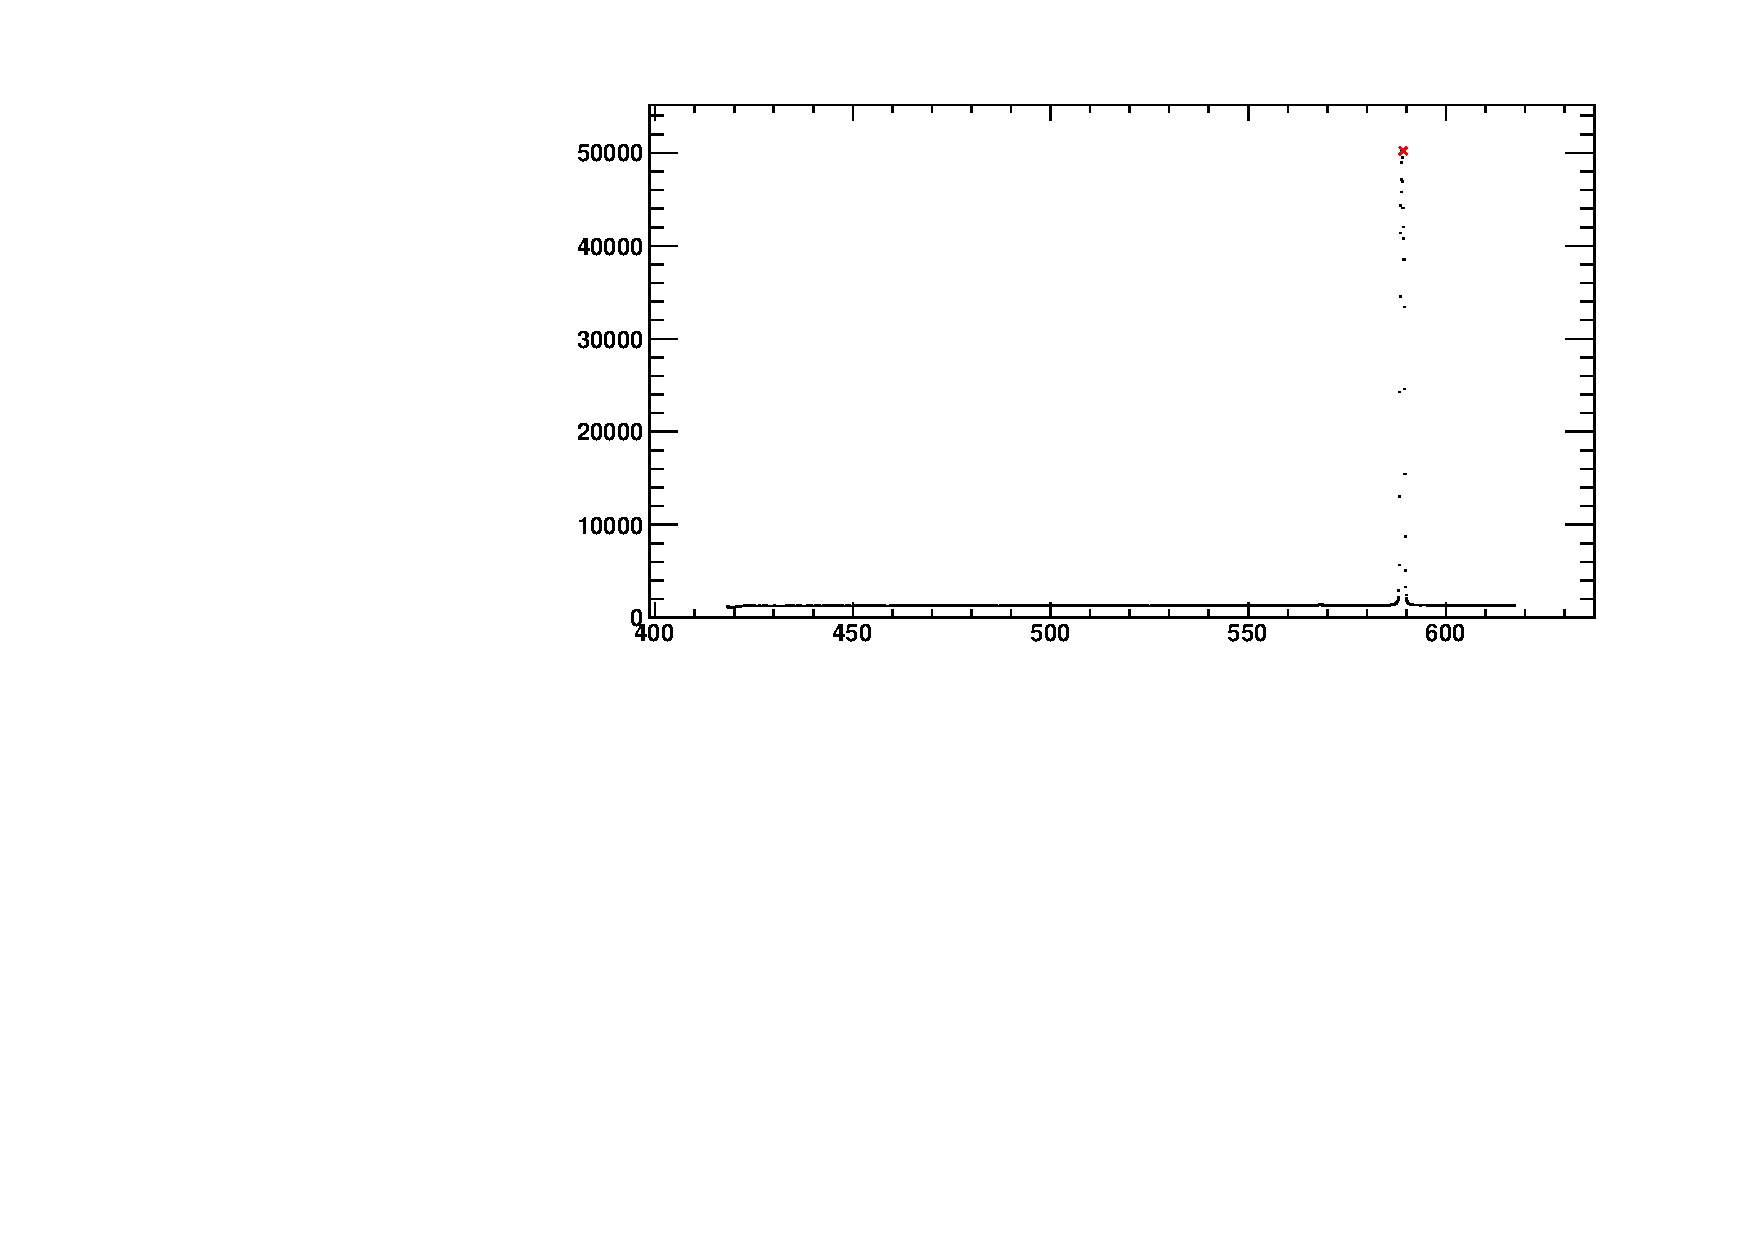
\includegraphics[width=\textwidth]{../img/NaPeaks.pdf}
  \caption[---]{Emission spectrum of Sodium with D-line at 589.20\,nm.}
  \label{img:na:spectrum}
\end{center}
\end{figure}

\begin{figure}[H]
\begin{center}
  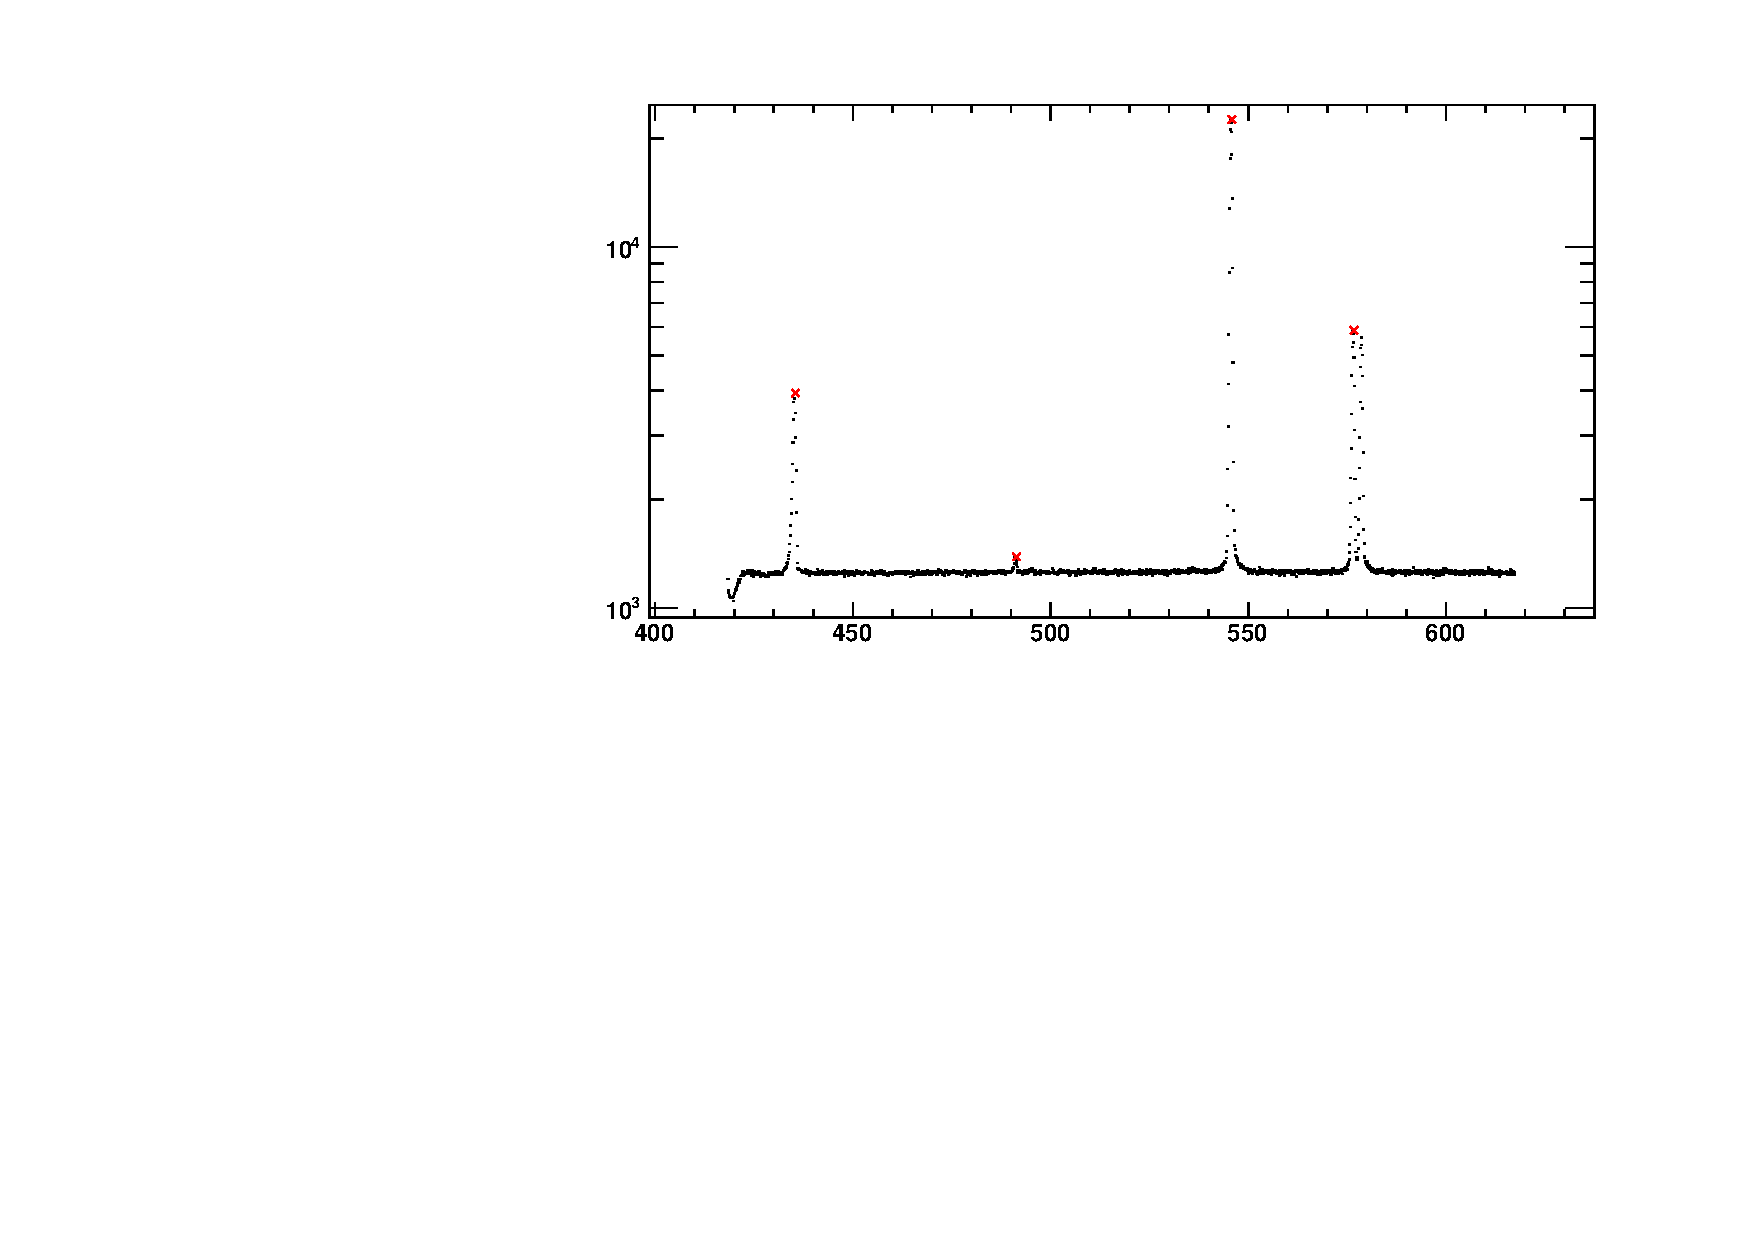
\includegraphics[width=\textwidth]{../img/HgPeaks.pdf}
  \caption[---]{Emission spectrum of Mercury with
  g-line at 435.83\,nm,
  e-line at 546.07\,nm and
  orange double lines at 576.96\,nm and 579.07\,nm.}
  \label{img:hg:spectrum}
\end{center}
\end{figure}

\begin{savenotes} % to catch footnotes in table
\begin{table}[H]
\caption{Measured and literature values for known lines of Mercury and Sodium}
\begin{center}
\begin{tabular}{|c|c|c|}
\hline
  Element & $\lambda_{\text{exp}}$ / nm & $\lambda_{\text{lit}}$ / nm \\ \hline
    Hg & 435.47 & 435.83 \\ \hline
    Hg & 491.38 & 491.61\footnote{Found at \url{http://physics.nist.gov/ASD}} \\ \hline
    Hg & 545.84 & 546.07 \\ \hline
    Hg & 576.73 & 576.96 \\ \hline
    Hg & 578.88 & 579.07 \\ \hline
    Na & 589.14 & 589.20\footnote{This is the weighted mean over the $D_1$- and $D_2$-line of Sodium, the weights are the relative intensities, also found at NIST} \\ \hline
\end{tabular}
\end{center}
\label{tab:energygauge}
\end{table}
\end{savenotes}

As you can see in \autoref{tab:energygauge} the measured data matches the literature values already well.
However, as a small offset is visible over the measured range, a linear fit has been done
to correct the data of the iodine absorption:
\begin{equation}
  \lambda_{\text{lit}} = a + b \cdot \lambda_{\text{exp}}
\end{equation}
The fit and the fitting parameters are shown on \autoref{img:calibrationsystem}. \\
Now an arbitrary measured wavelength $\lambda$ and its error can be corrected \footnote{The correlation coefficient between $a$ and $b$ is $\rho \approx -0.995$}:
\begin{equation}
  \lambda_{\text{corr}} = a + b \lambda, \qquad s_{\lambda_{\text{corr}}}^2 = 
  s_a^2 + \lambda^2 \cdot s_b^2 + b^2 \cdot s_\lambda^2 + 2 \cdot \lambda \cdot \rho \cdot s_a \cdot s_b
\end{equation}

\begin{figure}[H]
\begin{center}
  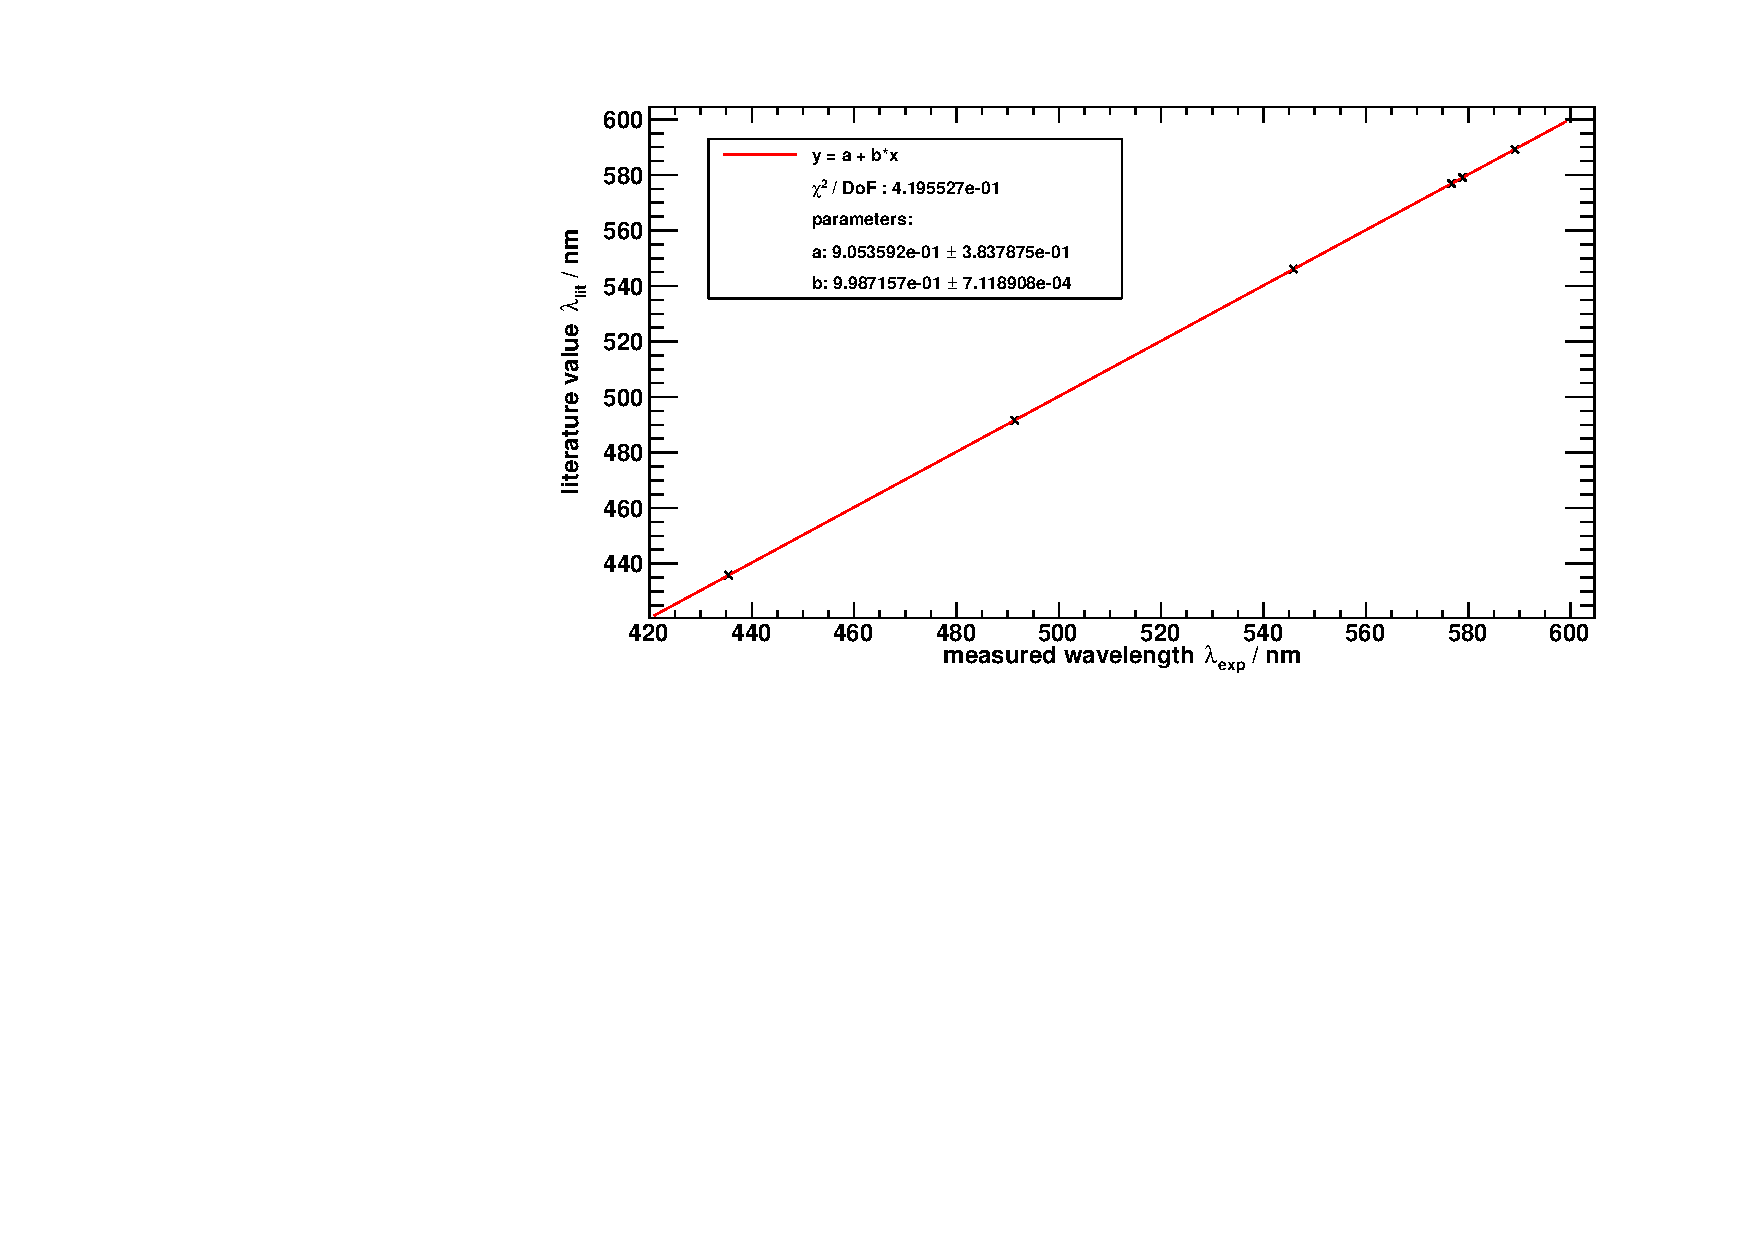
\includegraphics[width=\textwidth]{../img/energy_gauge.pdf}
  \caption[---]{Measured values for the lines of sodium and mercury versus literature values.
  The constant offset $a$ and the linear offset $b$ are used later to adjust the data of the iodine spectrum.}
  \label{img:calibrationsystem}
\end{center}
\end{figure}

Furthermore the shortening of the measured wavelengths, which is caused by air, needs to be considered.
\begin{equation}
  \lambda_{\text{vac}} = n(\lambda_{\text{air}}) \cdot \lambda_{\text{air}}
\end{equation}
Hence a linear fit on the literature values of the refractive index of air has been done (see \autoref{img:refindex}) and provides another
correcting function which is applied on the measured data for iodine:
\begin{equation}
  n(\lambda) = a + b \cdot \lambda
\end{equation}

\begin{figure}[H]
\begin{center}
  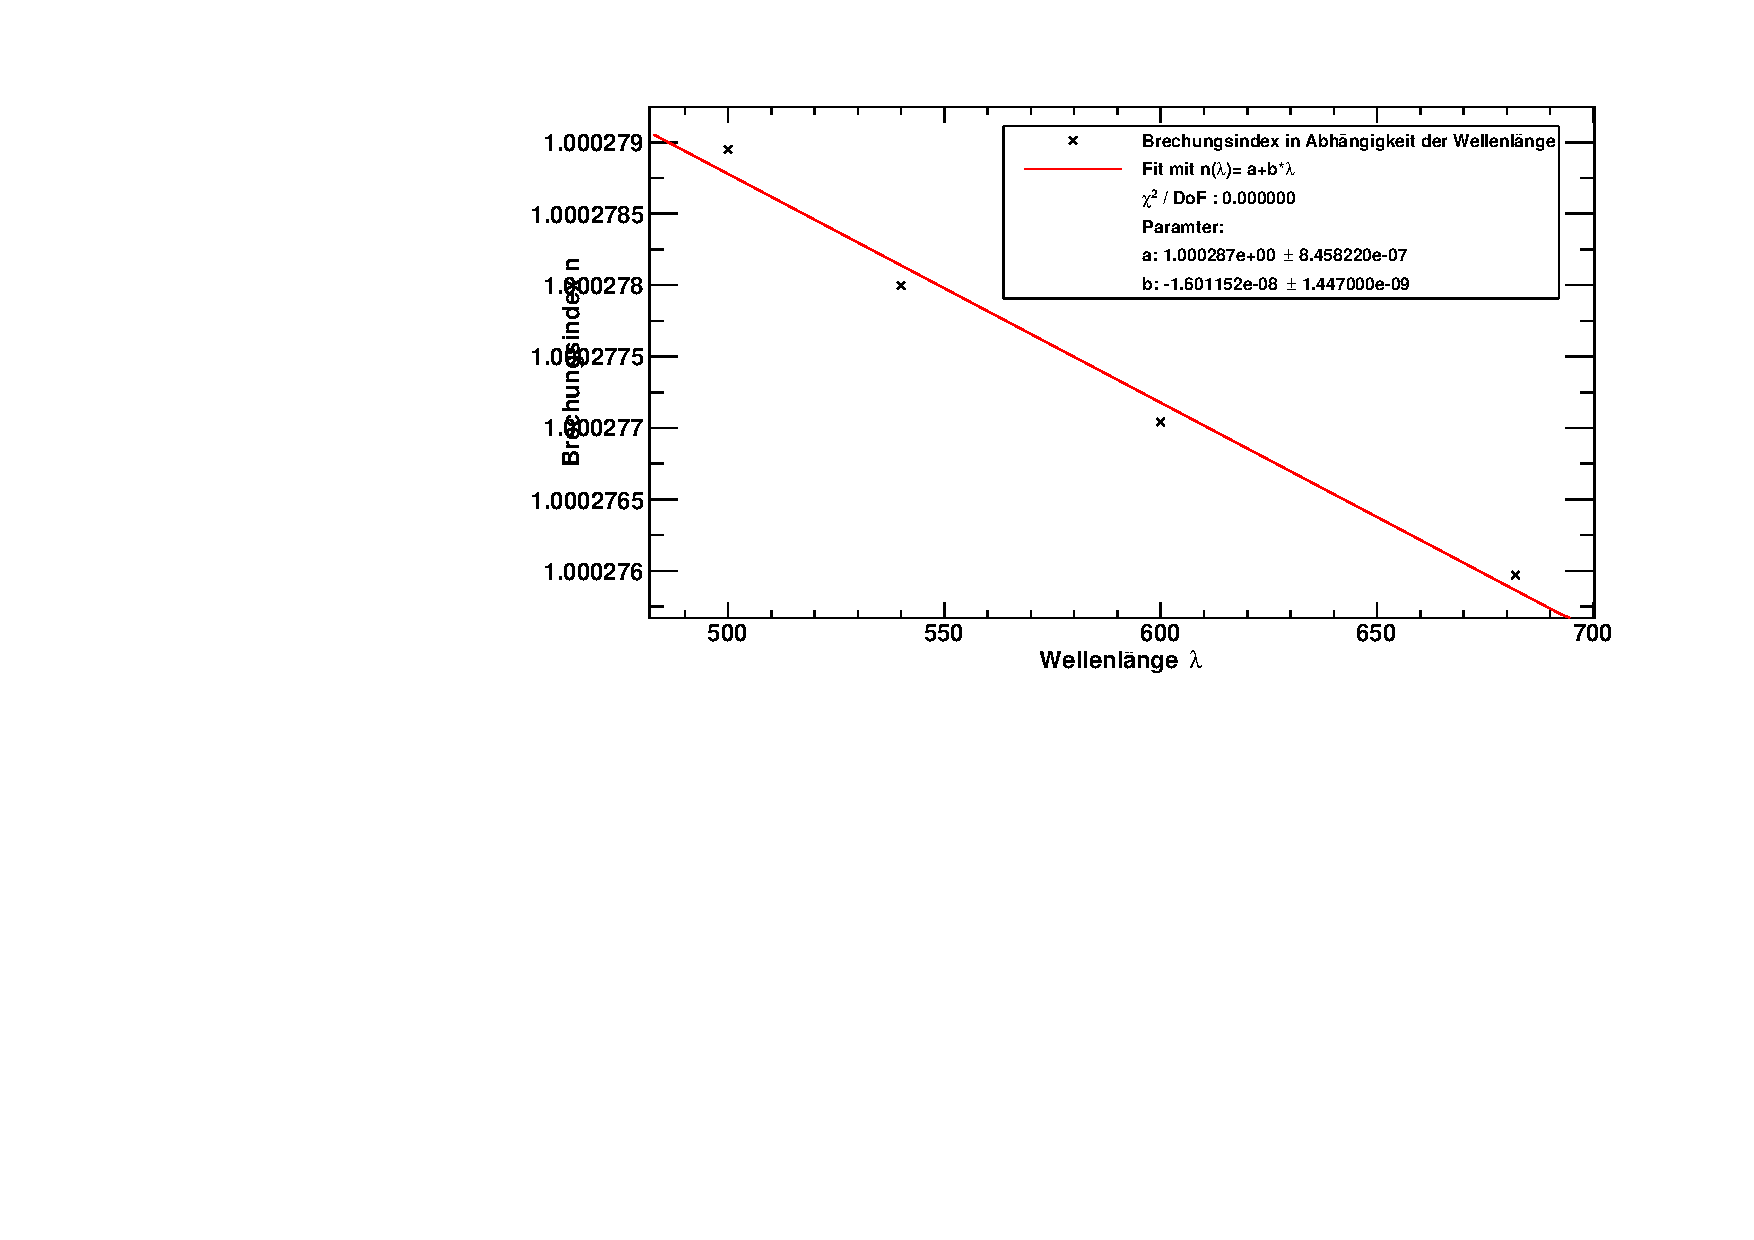
\includegraphics[width=\textwidth]{../img/fit_lambda.pdf}
  \caption[---]{Linear fit on the refraction index of air to obtain a function for adjusting
  the measured wavelengths to their vacuum value.}
  \label{img:refindex}
\end{center}
\end{figure}

With this correction a measured wavelength $\lambda$ in air can now be calculated as a vaccum wavelength\footnote{The correlation coefficient between $a$ and $b$ is $\rho \approx -0.993$}:
\begin{equation}
\begin{split}
  \lambda_{\text{vac}} &= a \cdot \lambda + b \cdot \lambda^2, \\
  s_{\lambda_{\text{vac}}}^2 &= 
  \lambda^2 \cdot s_a^2 + \lambda^4 \cdot s_b^2 + (a + 2 \cdot b \lambda)^2 s_{\lambda}^2 + 2 \cdot \lambda^3 \cdot \rho \cdot s_a \cdot s_b
\end{split}
\end{equation}




\subsection{Spectrum of the halogen lamp}

\autoref{img:hal:spectrum} shows the spectrum of the halogen lamp.
The spectrum looks smooth an no absorption lines are visible.
An approximation with the model of a black body gives no good description of the data,
so probably the emissivity of the lamp changes for different wavelengths. 



\begin{figure}[H]
\begin{center}
  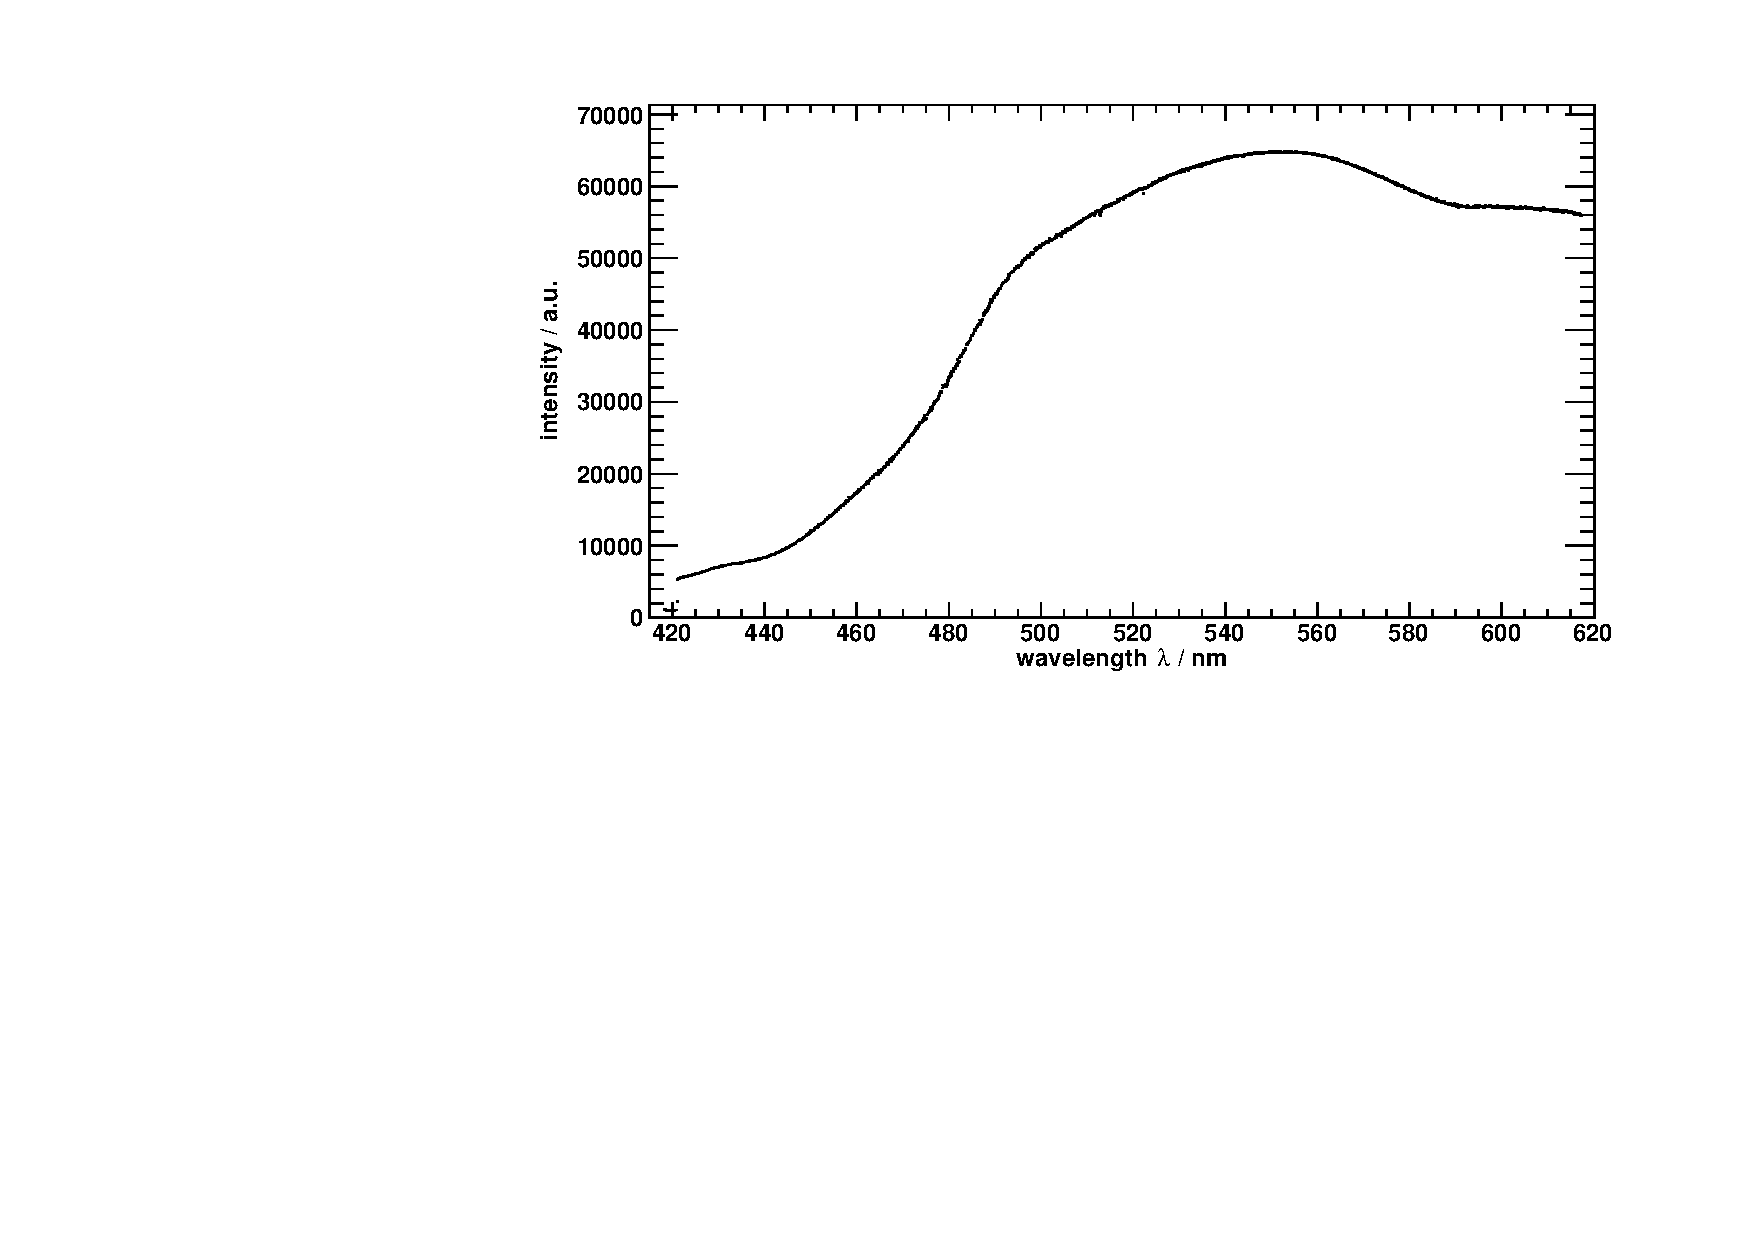
\includegraphics[width=\textwidth]{../img/halogen_lamp.pdf}
  \caption[---]{Spectrum of the halogen lamp.}
  \label{img:hal:spectrum}
\end{center}
\end{figure}




\subsection{Identification of the 3 progressions in the spectrum of iodine}

\begin{figure}[H]
\begin{center}
  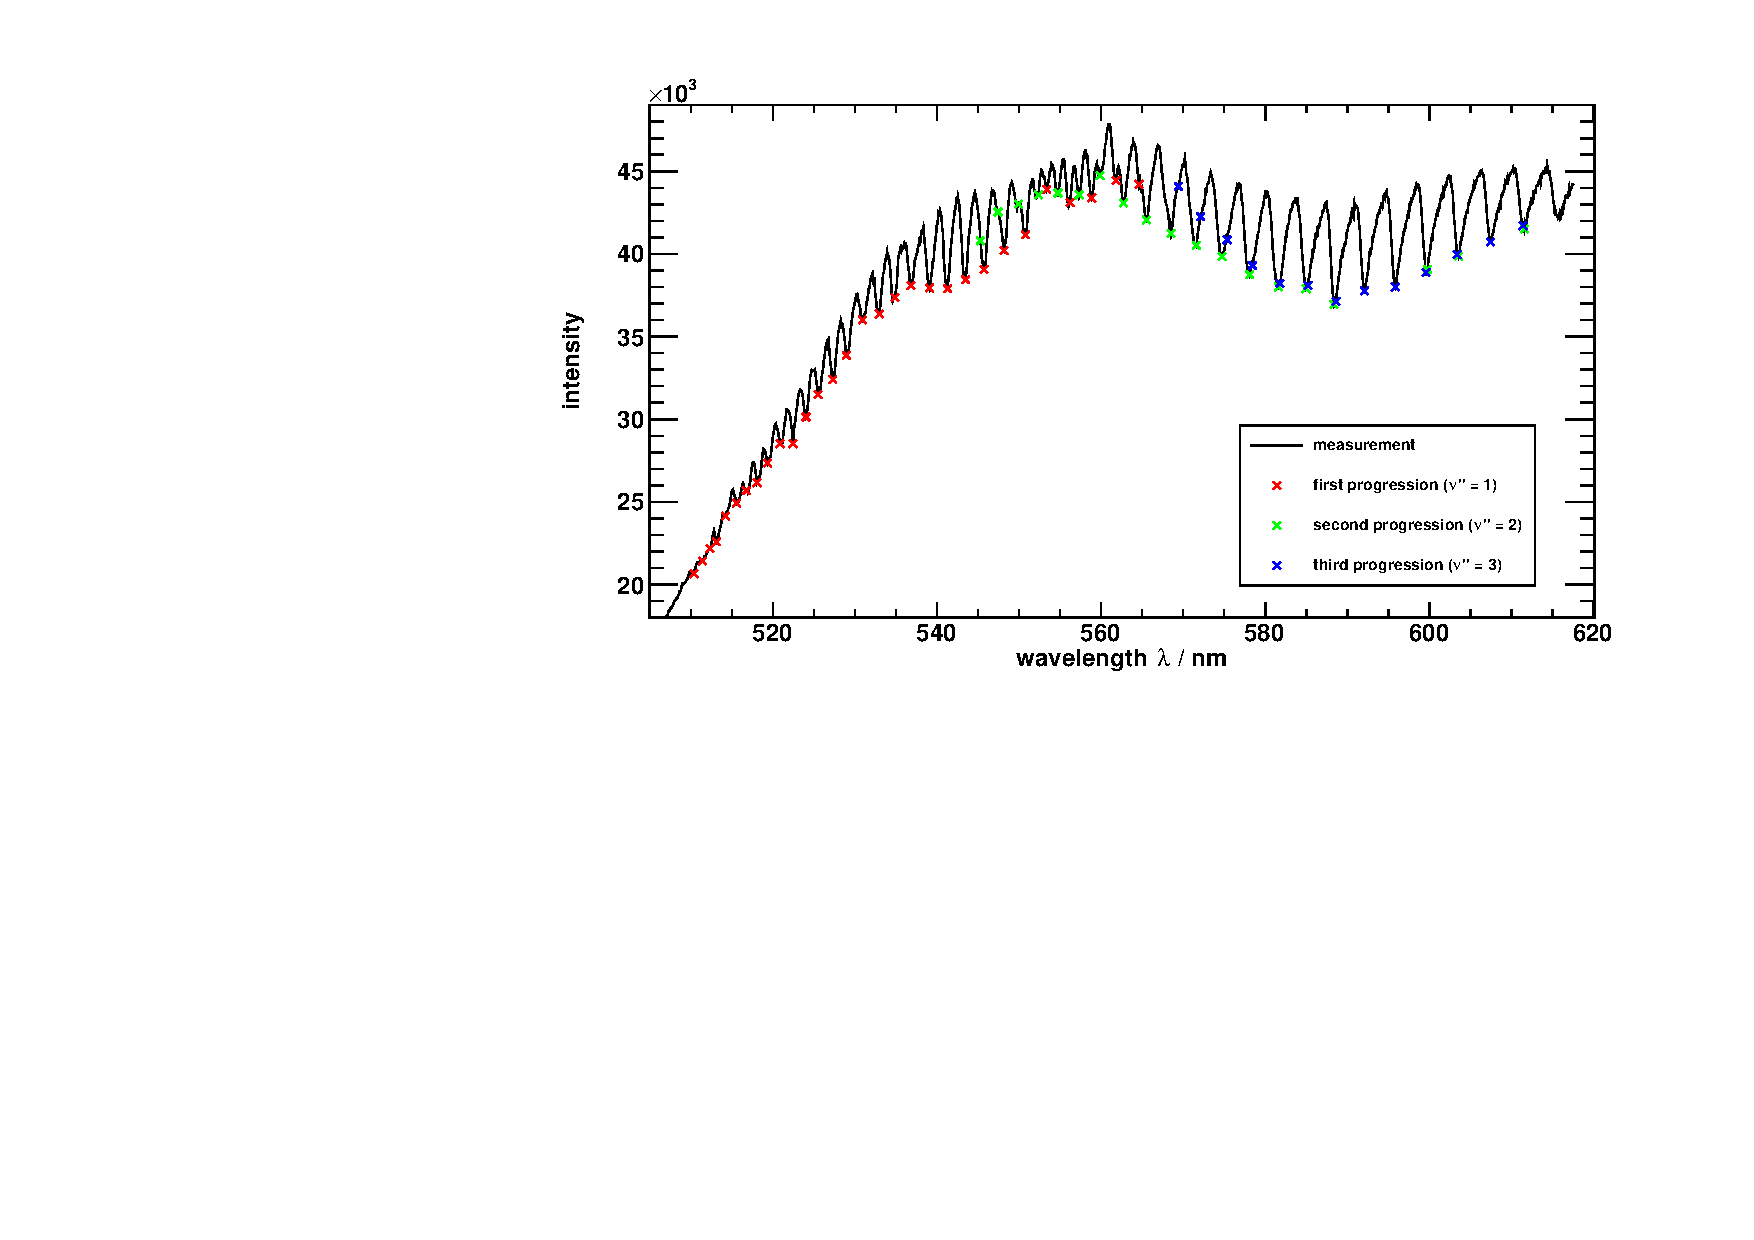
\includegraphics[width=\textwidth]{../img/I2_absorption.pdf}
  \caption[---]{Transmission spectrum of iodine and identification of absorption peaks due
  to electronic-vibronic transitions.}
  \label{img:spectrumiodine}
\end{center}
\end{figure}

\autoref{img:spectrumiodine} shows the measured transmission spectrum of a halogen lamp through iodine.
The first three progressions
(minima of transmission due to simultaneous electronic and vibronic excitation of iodine molecules)
could be identified and are marked in the
figure\footnote{The exact positions of the lines and
their corrected values (with calibration data of the setup and refraction index of air)
are shown in the Appendix, \autoref{tab:prog1}, \autoref{tab:prog2} and \autoref{tab:prog3}.}.
A closer look at the shape of those ''dips'' yields information about the ratio of the rotation constants
of the ground state and the excited electronic state:
The dips are slightly asymmetric and steeper on their left side. This so called
''red-shadowing'' appears, when the rotation constant of the excited state is \emph{smaller} than
the one of the ground state. As the constants are closely related to the equilibrium distance between the nuclei,
one can see that on excitation the nuclei move away from each other.

%TODO Nulllinie-Bandenkopf ???


\subsection{Evaluation of the vibration constants \texorpdfstring{$\omega_e'$}{we'} and \texorpdfstring{$\omega_e' x_e'$}{we'xe'} for the excited state via Birge-Sponer plots}
To make the Birge-Sponer plots,
the difference $\Delta G(\nu' +1/2)$ between two energy levels of one progression,
between $G(\nu' +1/2)$ and  $G(\nu' +3/2)$,
has been calculated with
\begin{equation}
  \Delta G(\nu' +1/2)=\frac{1}{\lambda_{\text{cor}}(\nu'+1)}-\frac{1}{\lambda_{\text{cor}}(\nu')}
\end{equation}
and
\begin{equation}
  s_{\Delta G(\nu' +1/2)}=
  \sqrt{\frac{s^2_{\lambda_{\text{cor}}(\nu'+1)}}{\lambda^4_{\text{cor}}(\nu'+1)}+
  \frac{s^2_{\lambda_{\text{cor}}(\nu')}}{\lambda^4_{\text{cor}}(\nu')}}
\end{equation}
The theoretical model for $\Delta G(\nu' +1/2)$ is given in \autoref{eq:iho:energydiff}:
\begin{equation}
  \Delta G(\nu' + \frac{1}{2})=\omega_e' - \omega_e' x_e'(2\nu'+2) + \omega_e' y_e'(3\nu'^2 + 6 \nu' +\frac{13}{4})
\end{equation}
This model was fitted on the data for the three progressions, as shown in \autoref{img:prog1},
\autoref{img:prog2} and \autoref{img:prog3}.

With the 2$^\text{nd}$-order model, there seems to appear a problem of overfitting,
particularly for the third progression.
So we decided to set the factor $\omega_e' y_e'$ to 0 and to use linear 1$^\text{st}$-order models
for further calculations.
The fitting parameters $\omega_e'$ and $\omega_e' x_e'$ we obtained from the three fits
are shown in \autoref{tab:prog1ord}.
\begin{table}[H]
\caption{Oscillation constants for first order fit of Birge-Sponer plots}
\begin{center}
\begin{tabular}{|c|c|c|c|c|}
  \hline
  $\nu''$ & $\omega_e' / \text{cm}^{-1}$ & $s_{\omega_e'} / \text{cm}^{-1}$ & $\omega_e' x_e' / \text{cm}^{-1}$ & $s_{\omega_e' x_e'} / \text{cm}^{-1}$ \\ \hline
  0 & 133.3 & 3.6 & 1.024 & 0.053 \\ \hline
  1 & 126.9 & 2.8 & 0.877 & 0.075 \\ \hline
  2 & 128.0 & 5.3 & 0.865 & 0.165 \\ \hline
\end{tabular}
\end{center}
\label{tab:prog1ord}
\end{table}

The weighted means (\autoref{eq:meanw}) of the values are
\begin{equation}
\begin{split}
    \overline{\omega_e'}		&   = (129.1 \pm 2.0)\,\text{cm}^{-1}\\
    \overline{\omega_e' x_e'} 	&	= (0.97 \pm 0.04)\,\text{cm}^{-1}
  \end{split}
\end{equation}
The literature values \cite{steinfeld} amount to
\begin{equation}
\begin{split}
    \omega_{e\text{,lit}}'			&   = 125.27\,\text{cm}^{-1}\\
    \omega_e' x_{e\text{,lit}}' 	&	= 0.702\,\text{cm}^{-1}
  \end{split}
\end{equation}
The first vibration constant $\overline{\omega_e'}$ includes the literature value within its 2-$\sigma$-interval, but
$\overline{\omega_e' x_e'}$ lies far away from the literature value. This could be caused by the rough
modelling in combination with not enough data points for the fit.



\begin{figure}[H]
\begin{center}
  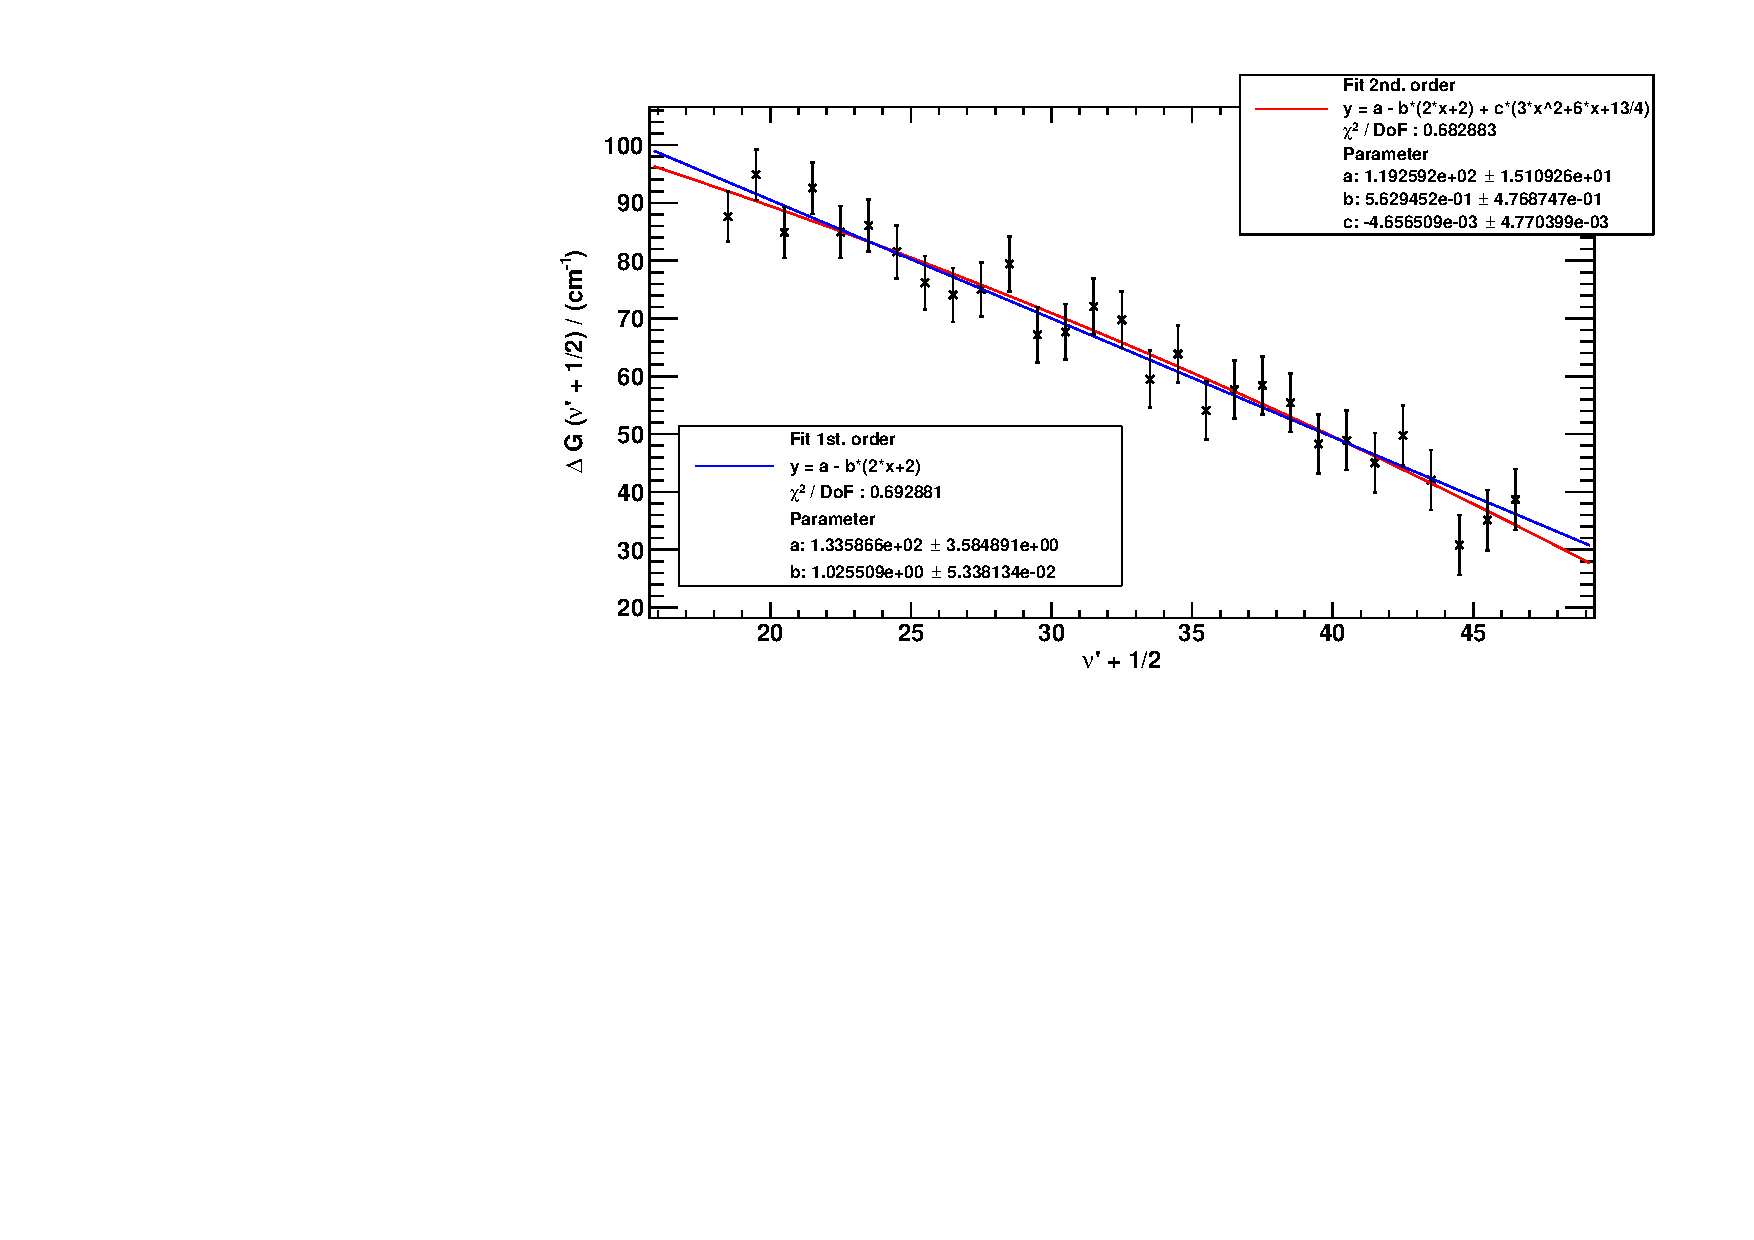
\includegraphics[width=\textwidth]{../img/prog1_birgesponer.pdf}
  \caption[---]{Birge-Sponer plot for the first progression and fits with models of linear and quadratic order.}
  \label{img:prog1}
\end{center}
\end{figure}


\begin{figure}[H]
\begin{center}
  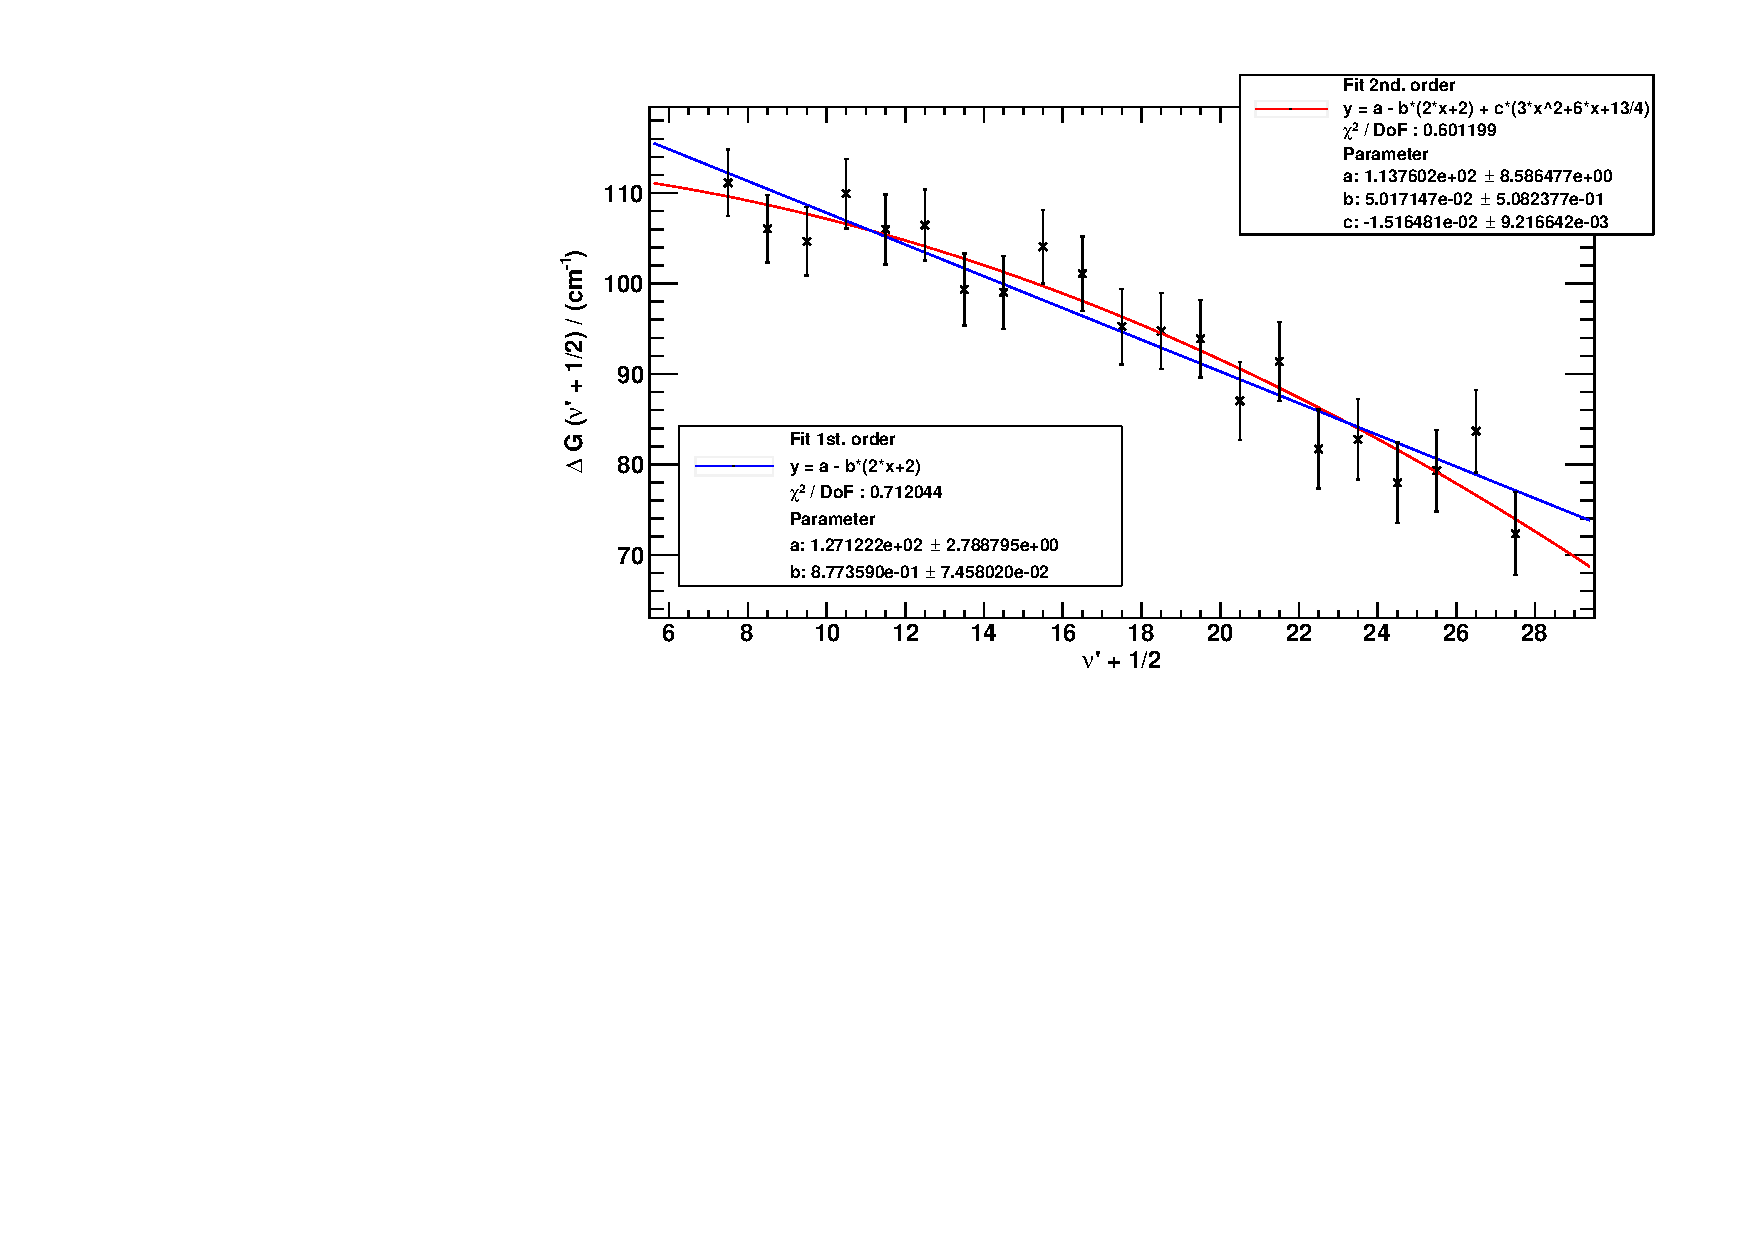
\includegraphics[width=\textwidth]{../img/prog2_birgesponer.pdf}
  \caption[---]{Birge-Sponer plot for the second progression and fits with models of linear and quadratic order.}
  \label{img:prog2}
\end{center}
\end{figure}


\begin{figure}[H]
\begin{center}
  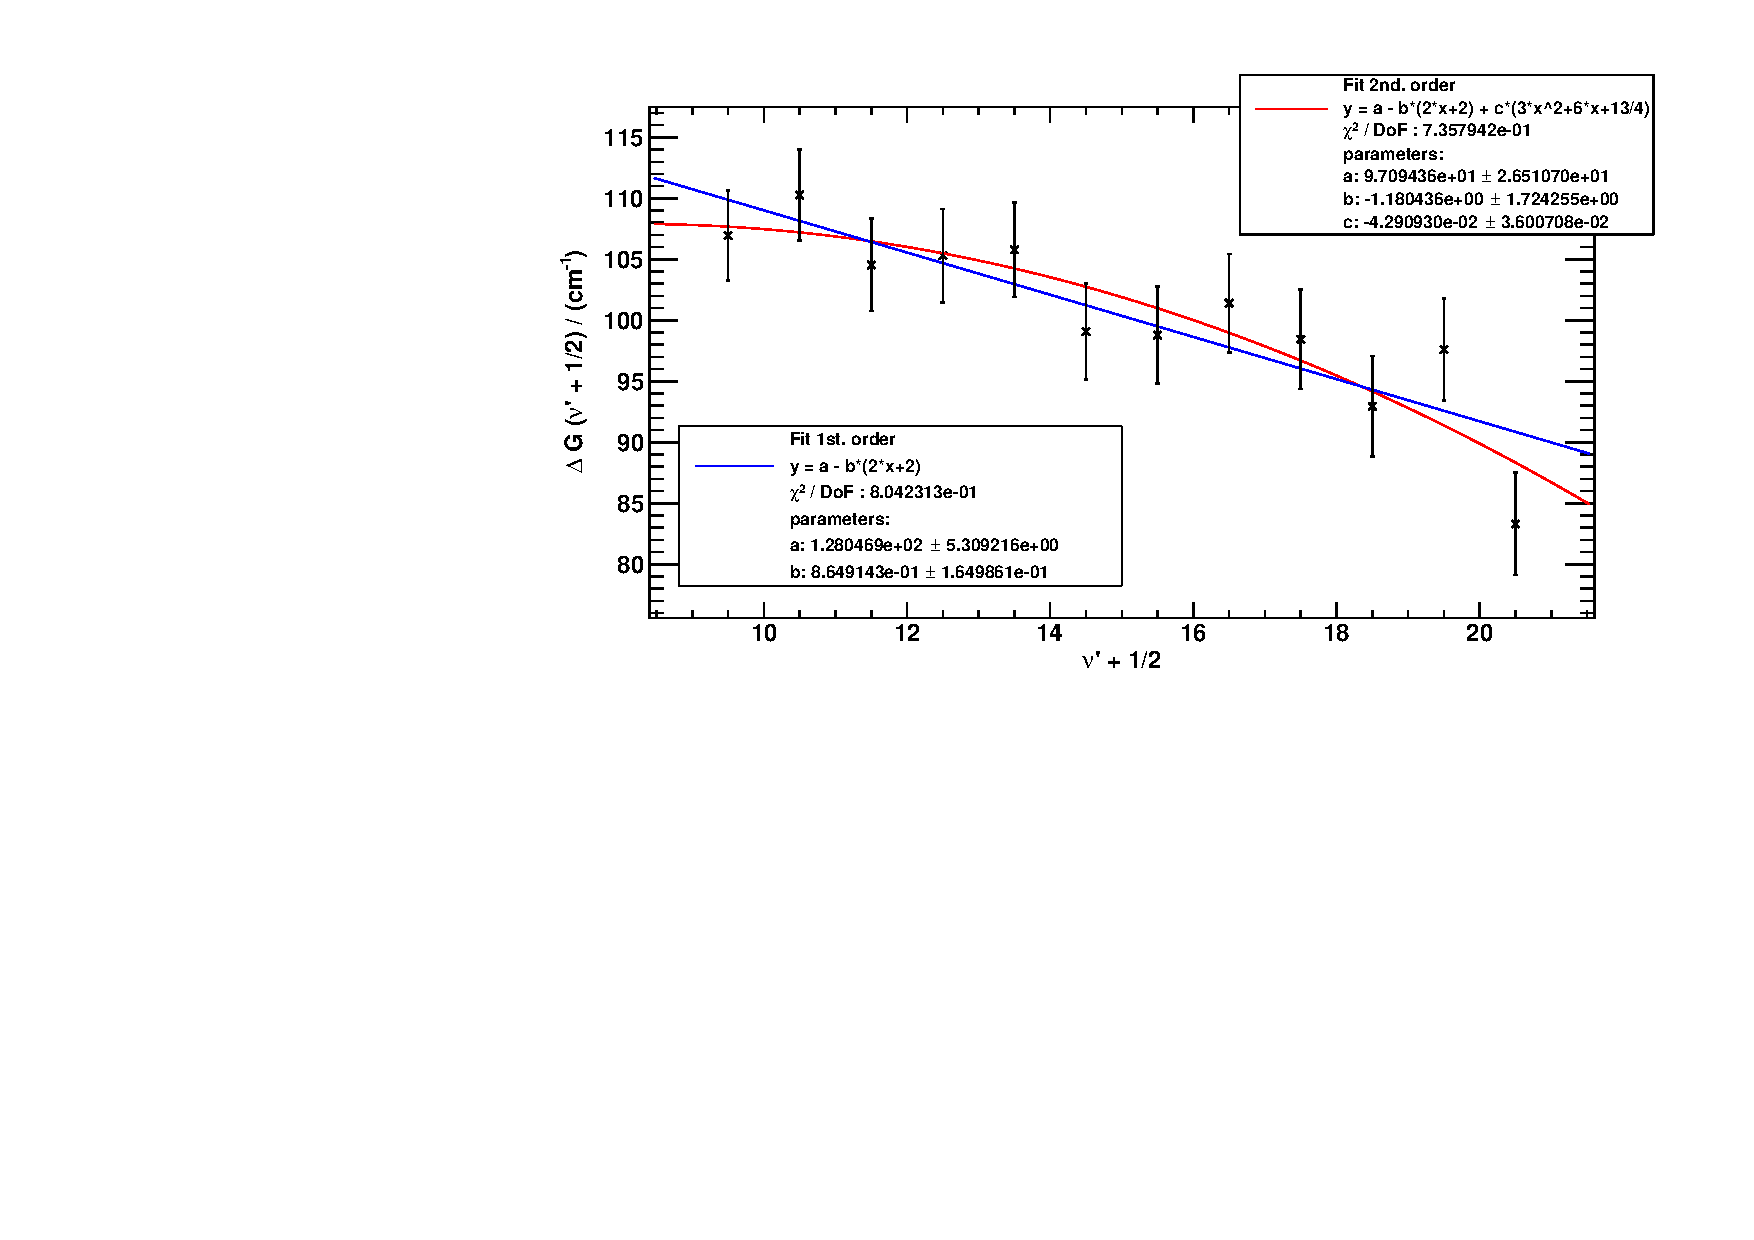
\includegraphics[width=\textwidth]{../img/prog3_birgesponer.pdf}
  \caption[---]{Birge-Sponer plot for the third progression and fits with models of linear and quadratic order.}
  \label{img:prog3}
\end{center}
\end{figure}


\subsection{Evaluation of the vibration constants \texorpdfstring{$\omega_e''$}{we''} and \texorpdfstring{$\omega_e'' x_e''$}{we''xe''} for the ground state}

\autoref{eq:iho:energydiff} states for the energy level $G''$ of the ground state
\begin{equation}
  G'' \left( \nu''+\frac{1}{2} \right) = \omega_e'' \left( \nu'' + \frac{1}{2} \right) - \omega_e'' x_e'' \left( \nu'' + \frac{1}{2} \right)^2 
\end{equation}
Due to the Boltzmann statistics, we only have data for the three lowest ground state levels
($\nu''=0,\nu''=1,\nu''=2$), which is
not enough for a proper fit like we could do with the excited state.
But we can express the energy differences between those levels by data we obtained from transitions
to the excited electronic state with the energy level $\nu'$:
\begin{equation}
\label{eq:DG}
\begin{split}
  \Delta G''\left( \frac{1}{2}\right)  &  =
   G''\left( \frac{3}{2}\right)-G''\left( \frac{1}{2}\right)   \\
 & = \left[G'\left(\nu'+\frac{1}{2}\right)-G''\left(\frac{1}{2}\right)\right]-
\left[G'\left(\nu'+\frac{1}{2}\right)-G''\left(\frac{3}{2}\right)\right]\\
& = \omega_e''-2\omega_e''x_e''\\
  \Delta G''\left( \frac{3}{2}\right)  &  =
   G''\left( \frac{5}{2}\right)-G''\left( \frac{3}{2}\right)\\
   & = \left[G'\left(\nu'+\frac{1}{2}\right)-G''\left(\frac{3}{2}\right)\right]-
\left[G'\left(\nu'+\frac{1}{2}\right)-G''\left(\frac{5}{2}\right)\right]\\
& = \omega_e''-4\omega_e''x_e''\\
  \end{split}
\end{equation}
We calculate the weighted mean (\autoref{eq:meanw}) of the values
we get for all the pairs in different progressions
with the same $\nu'$ in our measured data:
\begin{equation}
\begin{split}
 & \overline{\Delta G''(1/2)}= (211.83 \pm 1.34)\,\text{cm}^{-1}\\
 & \overline{\Delta G''(3/2)}= (208.87 \pm 1.11)\,\text{cm}^{-1}
 \end{split}
\end{equation}
Multiplying and adding the two expressions in \autoref{eq:DG}
gives us a way to calculate the two vibration constants:
\begin{equation}
\begin{split}
  \omega_e'' & =2\overline{\Delta G''(1/2)}- \overline{\Delta G''(3/2)}\\
  \omega_e''x_e'' & =\frac{1}{2}(\overline{\Delta G''(1/2)}- \overline{\Delta G''(3/2)})
  \end{split}
\end{equation}
To determine the errors we use the law of error propagation
\begin{equation}
\begin{split}
  s_{\omega_e''} & =\sqrt{4s^2_{\overline{\Delta G''(1/2)}}+ s^2_{\overline{\Delta G''(3/2)}}}\\
  s_{\omega_e''x_e''} & =\frac{1}{4}\sqrt{s^2_{\overline{\Delta G''(1/2)}}+ s^2_{\overline{\Delta G''(3/2)}}}
\end{split}
\end{equation}
The two equations above yield the results
\begin{equation}
\begin{split}
  \omega_e'' & =(215 \pm 3)\,\text{cm}^{-1}\\
  \omega_e''x_e'' & =(1.5 \pm 0.9)\,\text{cm}^{-1}
  \end{split}
\end{equation}
The literature values \cite{rank} are %TODO DO THAT!!!
\begin{equation}
\begin{split}
  \omega_{e\text{,lit}}'' & =214.5\,\text{cm}^{-1}\\
  \omega_e''x_{e\text{,lit}}'' & =0.61\,\text{cm}^{-1}
  \end{split}
\end{equation}
Our results match the literature values well. The high error on the second vibration constant
arises, because we use quite a crude way to get information about a subtle constant.



\subsection{Determination of the dissociation energies}

\subsubsection{Via Morse-Approximation for ground state and excited state}
Having evaluated the vibration constants in the last two sections, \autoref{eq:morse_dissenergy} gives us now a way
to calculate the dissociation energies for the ground state $D_e''$ and the excited state $D_e'$.
\begin{equation}
  D_e'' = \frac{\omega_e''^2}{4 \omega_e'' x_e''}= (8 \pm 5) \cdot 10^3\, \text{cm}^{-1}
\end{equation}
\begin{equation}
  D_e' = \frac{\omega_e'^2}{4 \omega_e' x_e'}= (43 \pm 2) \cdot 10^2\, \text{cm}^{-1}
\end{equation}
For the errors the following equation has been employed
\begin{equation}
  s_{D_e} = \frac{\omega_e \ \sqrt{4(\omega_e x_e)^2 \ s_{\omega_e}^2 + \omega_e^2 \ s_{\omega_e x_e}^2}}{4 (\omega_e x_e)^2}
\end{equation}
The literature values (from \cite{bitsch} and \cite{steinfeld}) for the dissociation energies are the following:
\begin{equation}
  D_{e,\text{lit}}''= 12560 \, \text{cm}^{-1}
\end{equation}
\begin{equation}
  D_{e,\text{lit}}' = 4391 \, \text{cm}^{-1}
\end{equation}
Our results match with the literature values.
The high error on the dissociation energy of the ground state is caused by the uncertainty
on the second vibration constant.

\subsubsection{Graphically from the Birge-Sponer plot for the excited state ($D_0'$)}
Calculating the dissociation energy $ D_0'$ of the excited state
is also possible with the data shown in \autoref{img:prog1}:
Summing up over all the
the energy differences $\Delta G'$ (\autoref{eq:dissenergy}) from the non-vibrating state ($\nu'=0$) up to the last
vibrational state ($\nu'=\nu'_{\text{diss}}$), from which, by further excitation, the molecule will separate:
\begin{equation}
\label{eq:dissenergy2}
  D_0' = \sum_{\nu'=0}^{\nu'_{\text{diss}}} \Delta G' \left( \nu' + \frac{1}{2} \right),
\end{equation}
As we do not have measurement values for $\nu'<18$ and $\nu'>47$,
we are forced to extrapolate to those values using our fitted model.
And since the fit was calculated with a least-square-approximation,
integrating the model over the range of the measured points should give a value
very close to the sum of the measured points.
So the equation above can be transformed into an integral form:
\begin{equation}
  D_0' = \int_{0}^{\nu'_{\text{diss}}} \Delta G'\left( \nu' + \frac{1}{2} \right) \difd \nu'
\end{equation}
Using our 1$^{\text{st}}$-order model, we get
\begin{equation}
D_0' = \int_{0}^{\nu'_{\text{diss}}} \omega_e' - \omega_e' x_e' (2\nu' + 2) \ \difd \nu'
\end{equation}
To find the $\nu'_{\text{diss}}$, we solve the equation
\begin{equation}
  \omega_e' - \omega_e' x_e' (2\nu'_{\text{diss}} + 2) = 0 \qquad \Leftrightarrow \qquad \nu'_{\text{diss}} =
  \frac{\omega_e'}{2\omega_e' x_e'} - 1
\end{equation}
This result is used to solve the integral:
\begin{equation}
  D_0' = \frac{(\omega_e'-2\omega_e' x_e')^2}{4\omega_e' x_e'}
\end{equation}
From the error propagation law we get
\begin{equation}
  s_{D_0'} = \frac
  {(\omega_e'-2\omega_e' x_e') \ \sqrt{4(\omega_e' x_e')^2 \ s_{\omega_e'}^2 + (\omega_e'+2\omega_e' x_e')^2 \ s_{\omega_e' x_e'}^2}}
  {4(\omega_e' x_e')^2}
\end{equation}
Using the data for the first progression (\autoref{tab:prog1ord}), we obtain the following value:
\begin{equation}
    D_0' = (42 \pm 3) \cdot 10^2\, \text{cm}^{-1}
    \end{equation}
This matches well the literature value \cite{steinfeld} for the dissociation energy $D_{0,\text{lit}}'$
\begin{equation}
  D_{0,\text{lit}}' = 4391 \, \text{cm}^{-1}
\end{equation}

\subsubsection{Analytically for the ground state ($D_0''$)}

Graphik mit Energieniveaus

\subsection{Determination of the energy for electronic excitation \texorpdfstring{$\sigma_{00}$}{s00}}

\subsection{Morse potential for the excited state}


\begin{figure}[H]
\begin{center}
  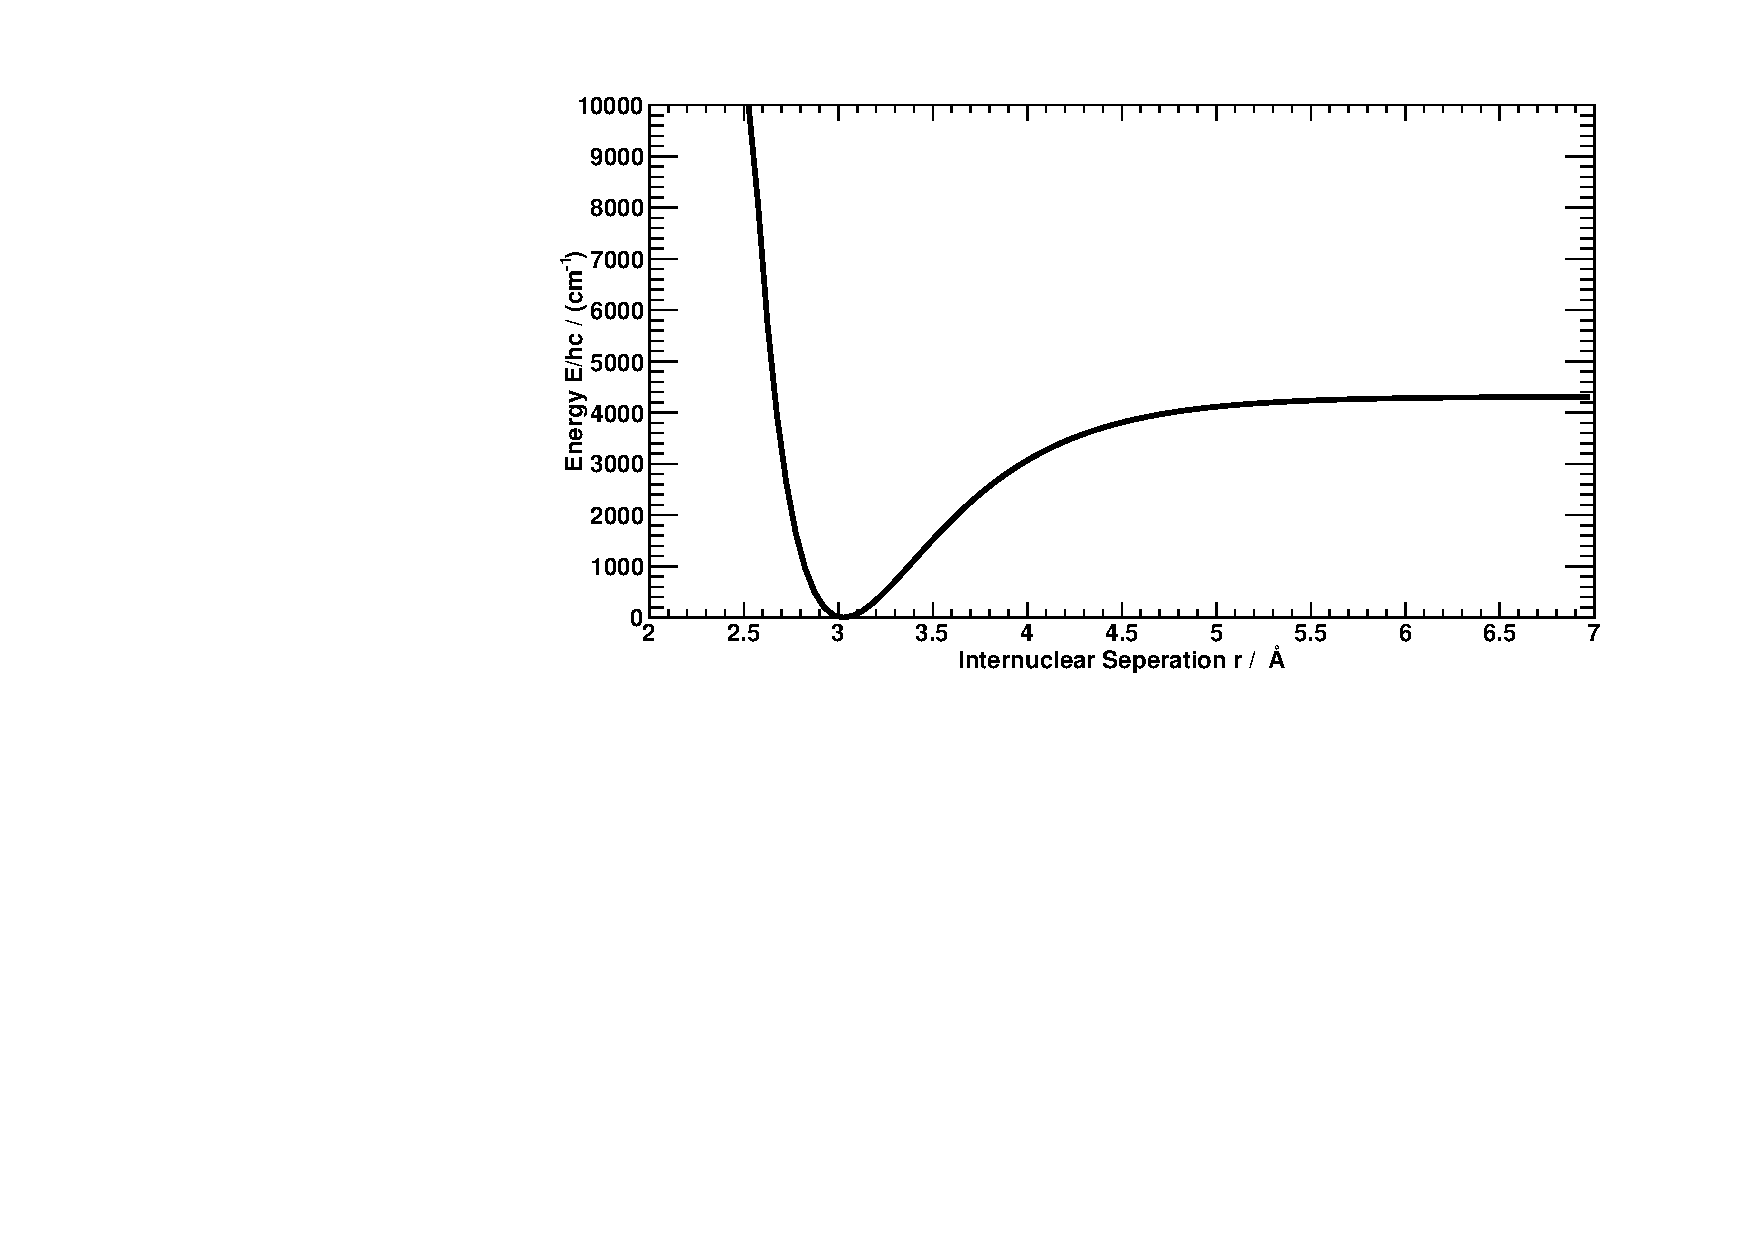
\includegraphics[width=\textwidth]{../img/morse.pdf}
  \caption[---]{---}
  \label{img:morse}
\end{center}
\end{figure}

